\section{Deep Learning against Misalignment}
\begin{frame}
\frametitle{Motivations (1)}
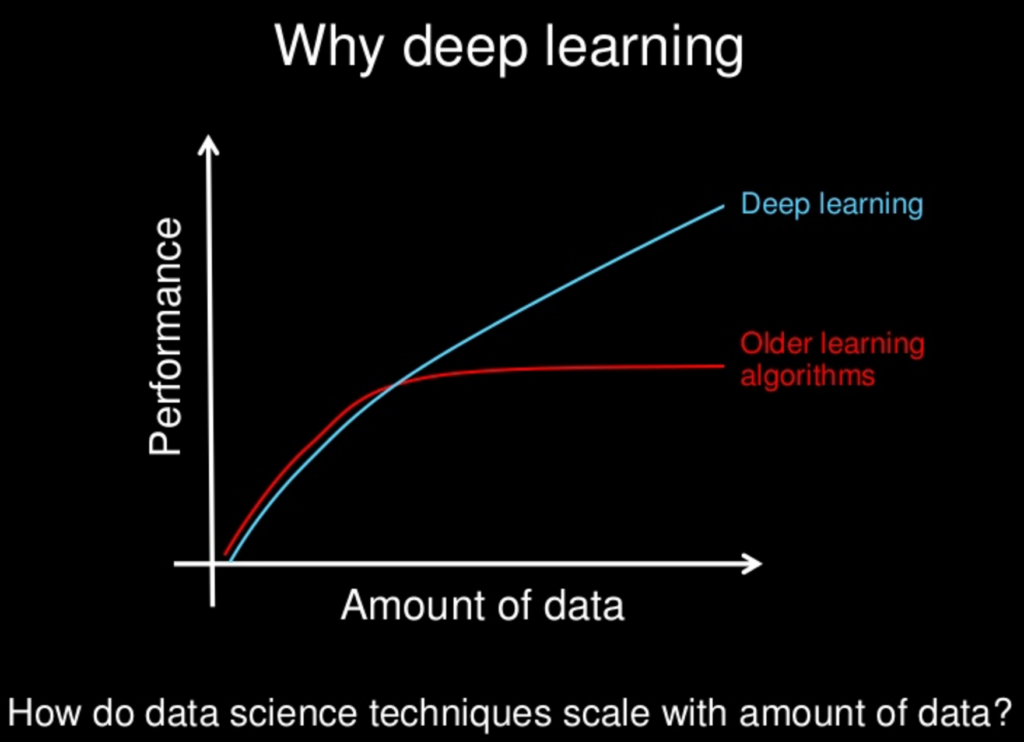
\includegraphics[width=.5\textwidth]{figures/whydeeplearning.png} 
\begin{itemize}
\item parallelizable computation(GPU optimizations)
\item not memory-based
\item many hyper-parameters but faster validation
\end{itemize}

\end{frame}

\begin{frame}
\frametitle{Motivations (2)}

\only<2->{
 \begin{textblock}{5}(5,5)
 \important{DEEP LEARNING}
 \end{textblock}
}
\textbf{Profiling phase}
\begin{itemize}
\item \only<1>{manage de-synchronization problem [$\setDataTrain \longrightarrow \rho\colon \mathbb{R}^D\rightarrow\mathbb{R}^D$]}\only<2->{\textcolor{gray}{manage de-synchronization problem [$\setDataTrain \longrightarrow \rho\colon \mathbb{R}^D\rightarrow\mathbb{R}^D$]}}
\item \only<1>{mandatory dimensionality reduction [$\setDataTrain \longrightarrow \extract\colon\mathbb{R}^D\rightarrow \mathbb{R}^C$]}
\only<2->{\textcolor{gray}{mandatory dimensionality reduction [$\setDataTrain \longrightarrow \extract\colon\mathbb{R}^D\rightarrow \mathbb{R}^C$]}}
\item estimate
\only<1>{
\begin{itemize}
\item $\pdf_{\given{\extract{(\rho(\vaLeakVec)})}{\sensRandVar = \sensVar}}$, $\pdf_{\extract{(\rho(\vaLeakVec)})}$, $\pdf_{\sensRandVar}$ (generative model)

\begin{itemize}
\item Gaussian hypothesis (\textbf{Template Attack})\cite{Chari2003}
\item Variants: \emph{pooled} version \cite{choudary2014efficient}, linear regression \cite{schindler2005stochastic}
\end{itemize}
\end{itemize}
}
\only<2->{
\begin{itemize}
\item \textcolor{gray}{$\pdf_{\given{\extract{(\rho(\vaLeakVec)})}{\sensRandVar = \sensVar}}$, $\pdf_{\extract{(\rho(\vaLeakVec)})}$, $\pdf_{\sensRandVar}$ (generative model)}
\begin{itemize}
\item \textcolor{gray}{ Gaussian hypothesis (\textbf{Template Attack})\cite{Chari2003}}
\item \textcolor{gray}{Variants: \emph{pooled} version \cite{choudary2014efficient}, linear regression \cite{schindler2005stochastic}}
\end{itemize}
\end{itemize}
}


\item $\pdf_{\given{\sensRandVar}{\only<1>{\extract{(\rho(\vLeakVec)}}  \only<2->{\vaLeakVec}}}$ (discriminative model) \\ \uncover<2->{by means of a neural network $F(\vaLeakVec)\approx \pdf_{\given{\sensRandVar}{ \only<2->{\vaLeakVec}}}$} 


\end{itemize}
\begin{block}{}
Many independent preprocessing steps and assumptions\\ \uncover<3>{$\longleftrightarrow$ integrated and agnostic approach}
\end{block}
\end{frame}


\begin{frame}
\frametitle{Multi-Layer Perceptron}
\hfill In SCA litterature \cite{martinasek2013optimization,martinasek2013innovative,martinasek2015profiling,martinasek2016profiling}
\begin{block}{Multi-Layer Perceptron (MLP)}
\only<1>{
$F(\vLeakVec,W) = \softmax\circ\lambda_n\circ\sigma_{n-1}\circ\lambda_{n-1}\circ\dots\circ \lambda_1(\vLeakVec)=\yyy \approx \mathrm{Pr}[\sensRandVar | \vaLeakVec = \vLeakVec] $
\begin{itemize}
\item[]\textcolor{white}{$\lambda_i$ linear functions (linear combinations of time samples) depending on some trainable weights $W$}
\item[]\textcolor{white}{$\sigma_i$ non-linear functions}
\item[]\textcolor{white}{$\softmax$ normalizing \emph{softmax} function}
\end{itemize}}
\only<2>{
$F(\vLeakVec,W) = \softmax\circ\textcolor{red}{\lambda_n}\circ\sigma_{n-1}\circ\textcolor{red}{\lambda_{n-1}}\circ\dots\circ \textcolor{red}{\lambda_1}(\vLeakVec)=\yyy \approx \mathrm{Pr}[\sensRandVar | \vaLeakVec = \vLeakVec]$
\begin{itemize}
\item[]\textcolor{red}{$\lambda_i$} linear functions (linear combinations of time samples) depending on some \textbf{trainable weights} $W$
\item[]\textcolor{white}{$\sigma_i$ non-linear functions}
\item[]\textcolor{white}{$\softmax$ normalizing \emph{softmax} function}
\end{itemize}}
\only<3>{
$F(\vLeakVec,W) = \softmax\circ\lambda_n\circ\textcolor{red}{\sigma_{n-1}}\circ\lambda_{n-1}\circ\dots\circ \lambda_1(\vLeakVec)=\yyy \approx \mathrm{Pr}[\sensRandVar | \vaLeakVec = \vLeakVec] $
\begin{itemize}
\item[]{$\lambda_i$ linear functions (linear combinations of time samples) depending on some \textbf{trainable weights} $W$}
\item[]\textcolor{red}{$\sigma_i$} non-linear \emph{activation} functions
\item[]\textcolor{white}{$\softmax$ normalizing \emph{softmax} function}
\end{itemize}}
\only<4->{
$F(\vLeakVec,W) = \textcolor{red}{\softmax}\circ\lambda_n\circ\sigma_{n-1}\circ\lambda_{n-1}\circ\dots\circ \lambda_1(\vLeakVec)=\yyy \approx \mathrm{Pr}[\sensRandVar | \vaLeakVec = \vLeakVec] $
\begin{itemize}
\item[]{$\lambda_i$ linear functions (linear combinations of time samples) depending on some \textbf{trainable weights} $W$}
\item[]{$\sigma_i$ non-linear \emph{activation} functions}
\item[]\textcolor{red}{$\softmax$} normalizing \emph{softmax} function \uncover<5->{\hfill Architecture hyper-parameters}
\end{itemize}}

\end{block}
%\uncover<5->{
%\begin{block}{Softmax $\sim$ multi-class logistic sigmoid}
%\begin{equation}\label{eq:softmax}
%\softmax(\aaa)[k] = \frac{e^{\aaa[k]}}{\sum_{j=1}^{\numClasses}e^{\aaa[j]}}\mbox{ .}
%\end{equation}
%\begin{equation}\label{eq:post_probs_multi-class}
%\prob(\given{\sensVarValue{j}}{\vLeakVec})  = \frac{\prob(\given{\vLeakVec}{\sensVarValue{j}})\prob(\sensVarValue{j})}{\prob(\vLeakVec)} = \frac{\prob(\given{\vLeakVec}{\sensVarValue{j}})\prob(\sensVarValue{j})}{\sum_{k=1}^{\nbClasses}\prob(\given{\vLeakVec}{\sensVarValue{k}})\prob(\sensVarValue{k} )} = \softmax (\aaa)[j]\mbox{ ,}
%\end{equation}
%\end{block}
%}
\uncover<6->{Universal approximation theorem}
\hfill \uncover<2->{
\begin{figure}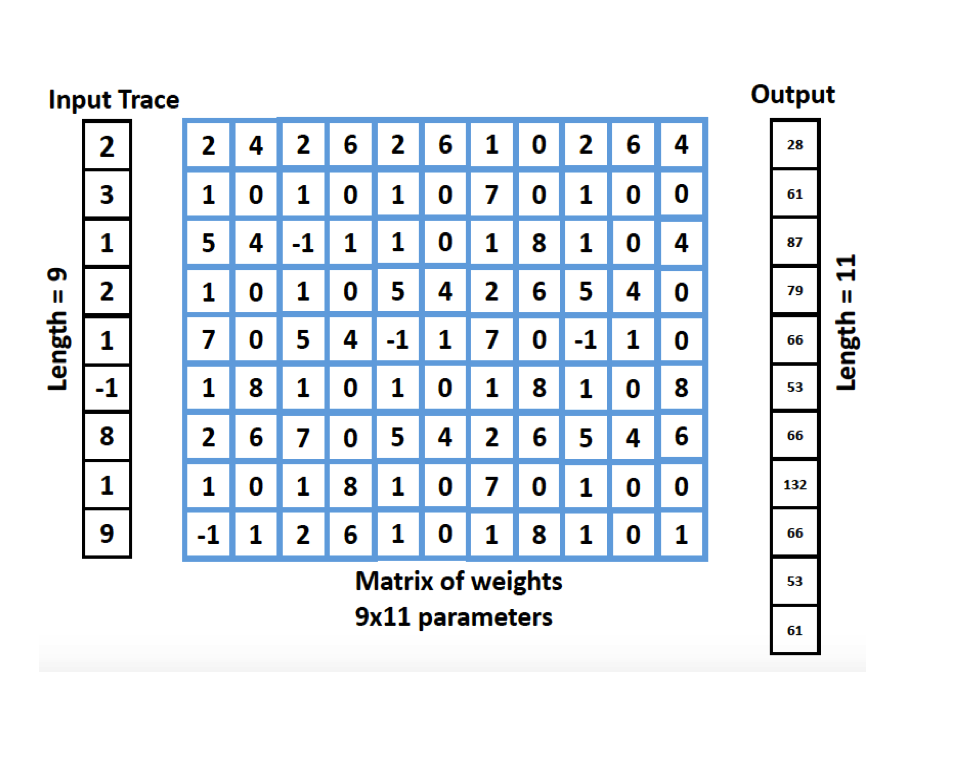
\includegraphics[width=.35\textwidth]{Figures/FC_si.png}}
\caption{\scriptsize{Linear layer in an MLP (\emph{Fully Connected Layer})}}
\end{figure}
\end{frame}

\begin{frame}
\frametitle{Convolutional Neural Networks}
\vspace*{-10pt}
\begin{block}{Translation-invariance}
\begin{figure}
\centering
\only<1>{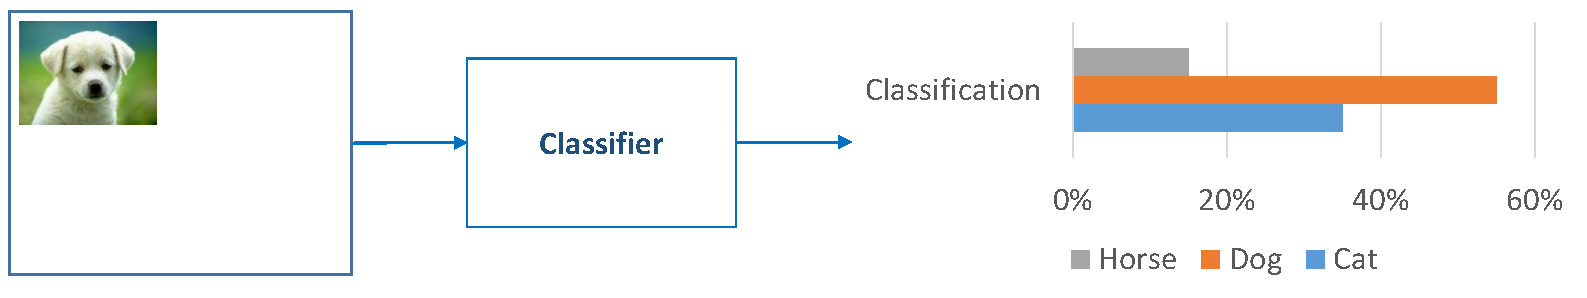
\includegraphics[width=\textwidth]{Figures/cane_shift_classifier1.pdf}}
\only<2>{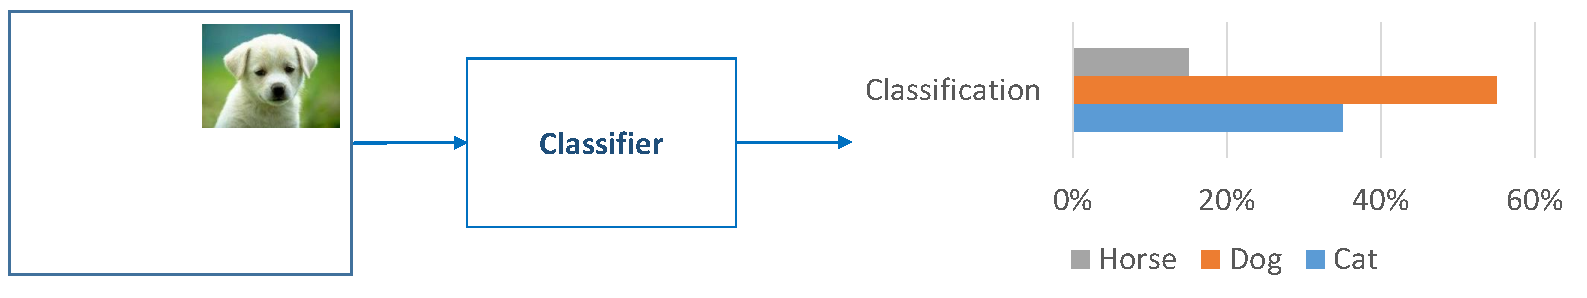
\includegraphics[width=\textwidth]{Figures/cane_shift_classifier2.pdf}}
\only<3-4>{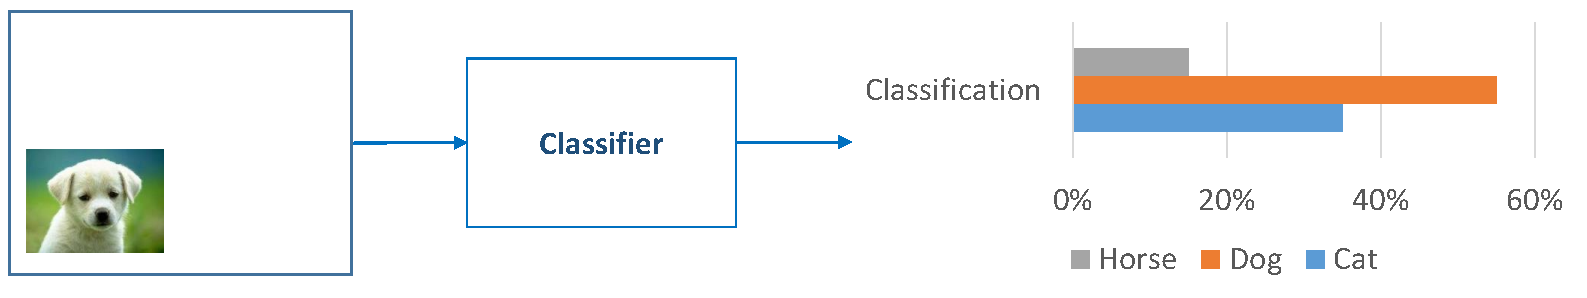
\includegraphics[width=\textwidth]{Figures/cane_shift_classifier3.pdf}}
%\only<5>{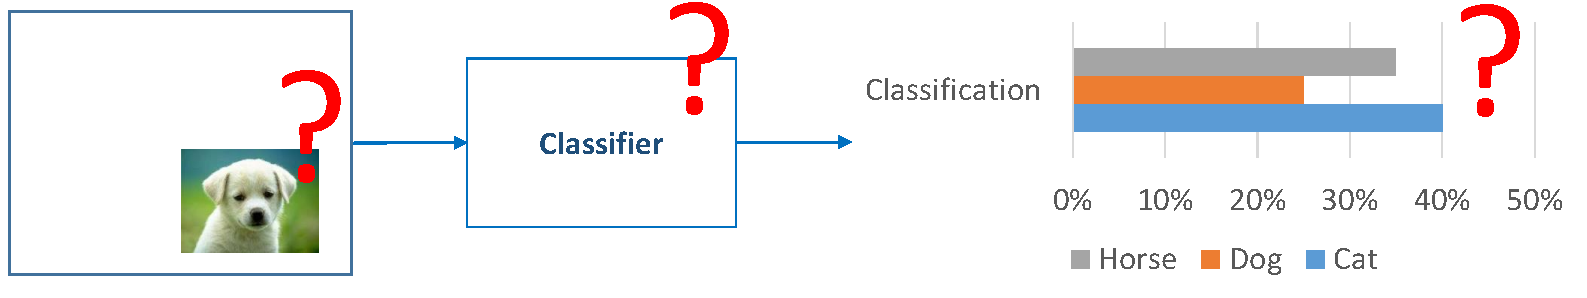
\includegraphics[width=\textwidth]{Figures/cane_shift_classifier4.pdf}}
\only<5>{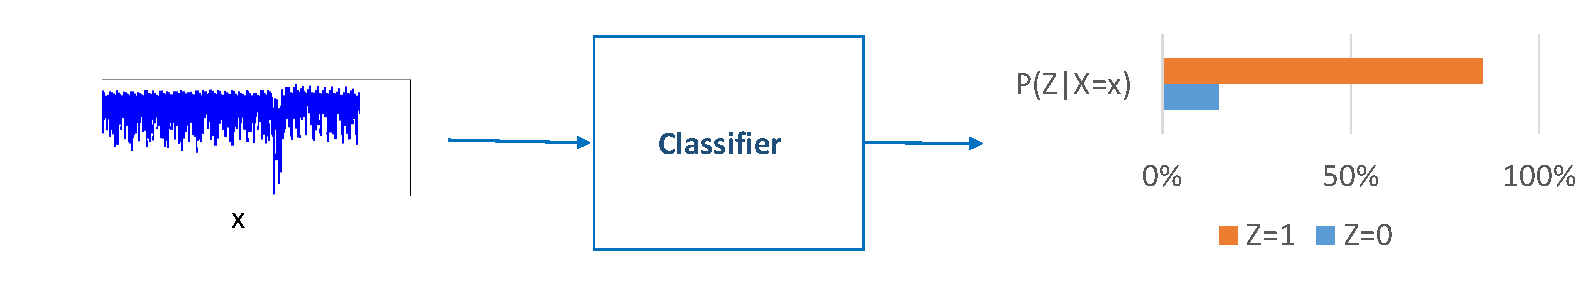
\includegraphics[width=\textwidth]{Figures/trace_shift_classifier1.pdf}}
\only<6>{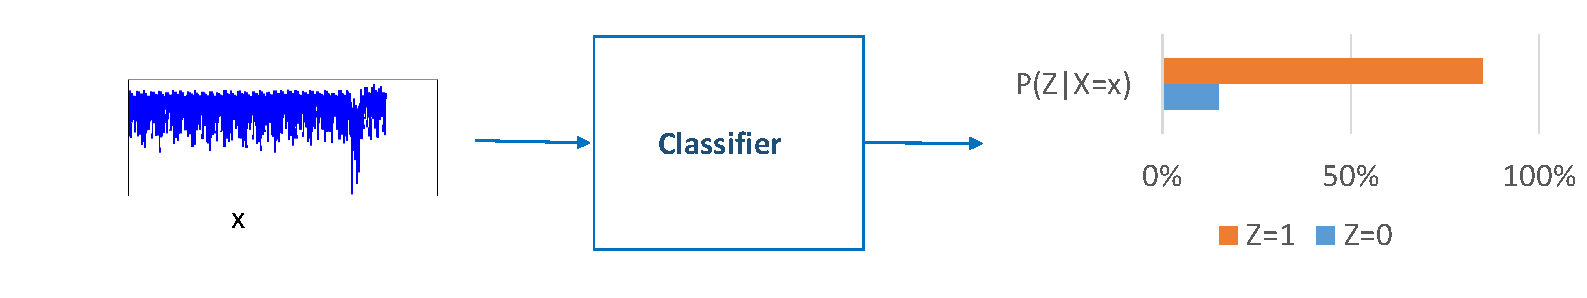
\includegraphics[width=\textwidth]{Figures/trace_shift_classifier2.pdf}}
\only<7->{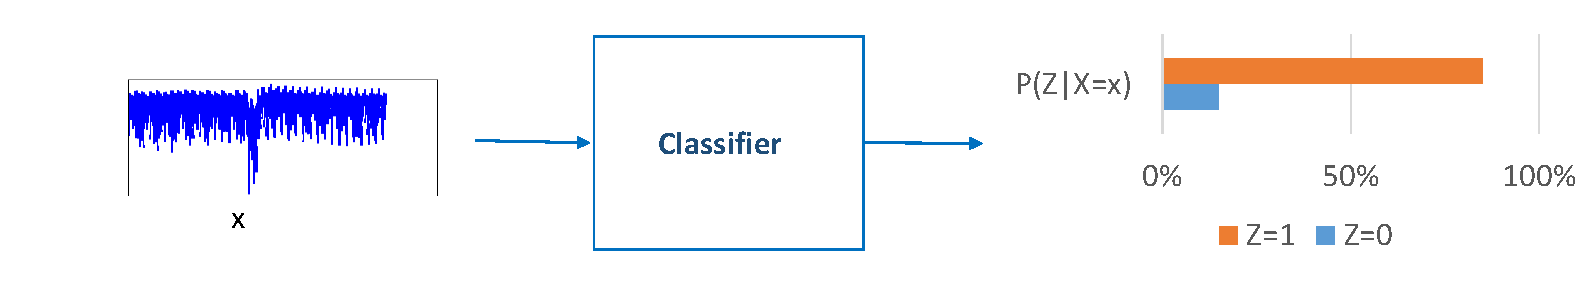
\includegraphics[width=\textwidth]{Figures/trace_shift_classifier3.pdf}}
\end{figure}
\uncover<4->{It is important to explicit the data translation-invariance\\}
\uncover<9->{Convolutional Neural Networks: share weights across space}
\end{block}
%

\vspace*{-7pt}

\begin{columns}
\begin{column}{.5\textwidth}
\only<1-10>{
\begin{figure}

\includegraphics[width=.7\textwidth]{Figures/small_white.pdf}
\end{figure}
}

\only<11>{
\begin{figure}
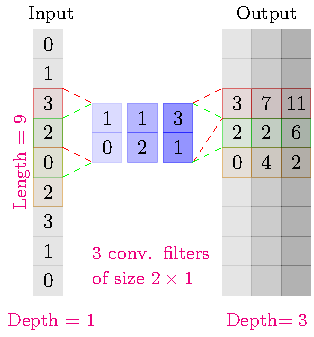
\includegraphics[width=.5\textwidth]{../tikz_per_manuscritto/conv_filter_2_1.pdf} 
\caption{\scriptsize{Linear layer in a ConvNet (\emph{Convolutional Layer})}}
\end{figure}
}

\only<12-13>{
\begin{figure}
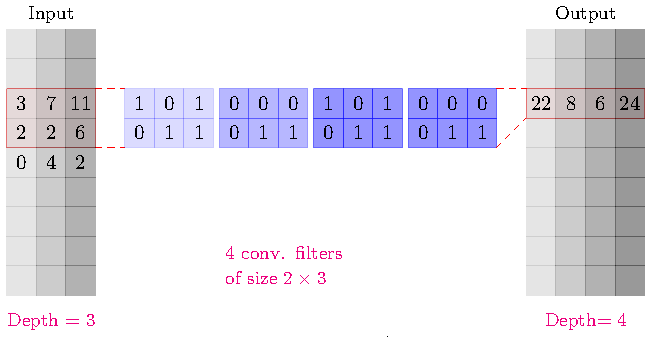
\includegraphics[width=0.8\textwidth]{../tikz_per_manuscritto/conv_filter_2_3.pdf} 
\caption{\scriptsize{Linear layer in a ConvNet (\emph{Convolutional Layer})}}
\end{figure}
}

\end{column}
%%
\begin{column}{.5\textwidth}
\only<1-9>{
\begin{figure}

\includegraphics[width=.7\textwidth]{Figures/big_white.pdf}
\end{figure}}
\only<10-12>{
\begin{figure}
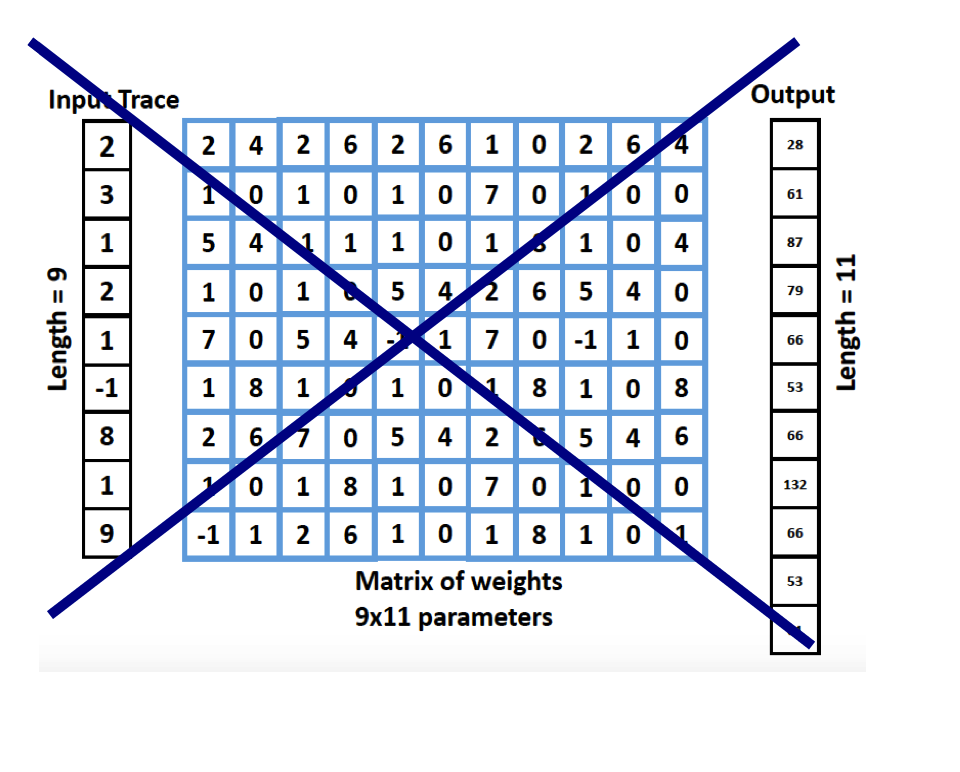
\includegraphics[width=.7\textwidth]{Figures/FC_no.png} 
\caption{\scriptsize{Linear layer in an MLP (\emph{Fully Connected Layer})}}
\end{figure}
}
\only<13->{
\begin{figure}
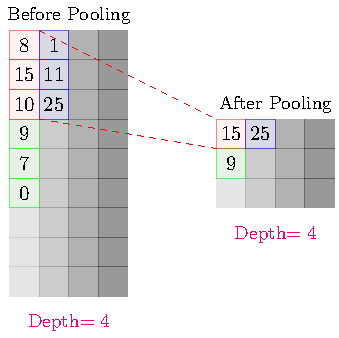
\includegraphics[width=.5\textwidth]{../tikz_per_manuscritto/pooling.pdf} 
\caption{\scriptsize{Max Pooling Layer}}
\end{figure}
}

\end{column}
\end{columns}
\end{frame}


\begin{frame}
\frametitle{A kind of CNN architecture}
\vspace*{-10pt}
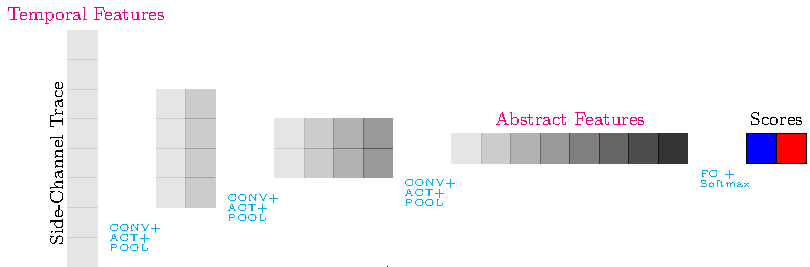
\includegraphics[width=0.8\textwidth]{../tikz_per_manuscritto/convnet_arch.pdf} \\
Architecture inspired by AlexNet \cite{KSH12}, VGG \cite{simonyan2014very}, ResNet \cite{he2016deep} design rules:
\begin{itemize}
\item Reduce temporal features to only one
\item Maintain time complexity of each layer (one-half pooling when number of feature maps are doubled)
\item Small filters
\end{itemize}
\begin{block}{Model used in our experiments}
\begin{itemize}
\item 4 Conv + Pool layers
\item tanh activations
\item batch normalisation \cite{batch_norm}
\item 1 \emph{fully connected layer} + softmax
\end{itemize}
\end{block}

\end{frame}

%\begin{frame}
%
%\frametitle{Training and overfitting}
%%\vspace{-12pt}
%%\begin{block}{Training and validation set}
%%
%% Profiling set 
%%$\rightarrow
%%\begin{cases} \mathrm{Training\ set}\\
%% \mathrm{Validation\ set}
%% \end{cases}$
%%
%%\end{block}
%\vspace{-12pt}
%\begin{block}{Training}
%\begin{itemize}
%\item[]  Profiling set 
%$\rightarrow
%\begin{cases} \mathrm{Training\ set}\\
% \mathrm{Validation\ set}
% \end{cases}$
%\item[] Randomly partition training set into batches
%\item[] Iterative optimization algorithm over batches (cost function, stochastic gradient descent)
%\item[] \emph{Epoch}:= one pass over the entire training set
%
%\end{itemize}
%
%\end{block}
%\pause
%\begin{block}{ Evaluate and compare training and validation accuracy}
%\begin{columns}
%\begin{column}{.45\textwidth}
%\only<2>{Understand significant features
%\begin{figure}
%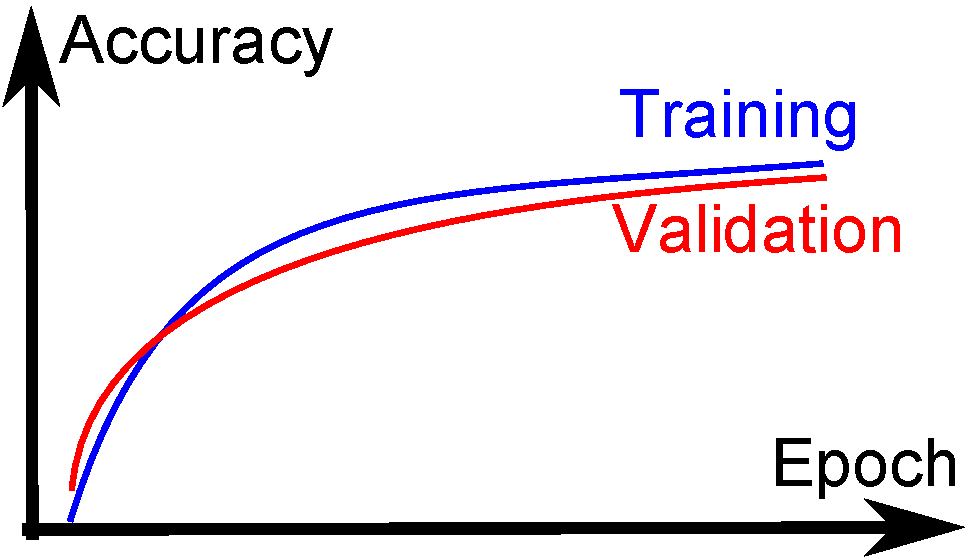
\includegraphics[width=.9\textwidth]{Figures/fitting.pdf} 
%\end{figure}
%}
%\only<3>{
%Why?
%\begin{itemize}
%\item[] Too complex model
%\item[] Not enough training data
%\end{itemize}
%Solution? 
%\begin{itemize}
%\item[] Data augmentation
%\end{itemize}
%}
%\end{column}
%\begin{column}{.45\textwidth}
%Learn by heart (\textbf{\textcolor{red}{OVERFITTING}})
%\begin{figure}
%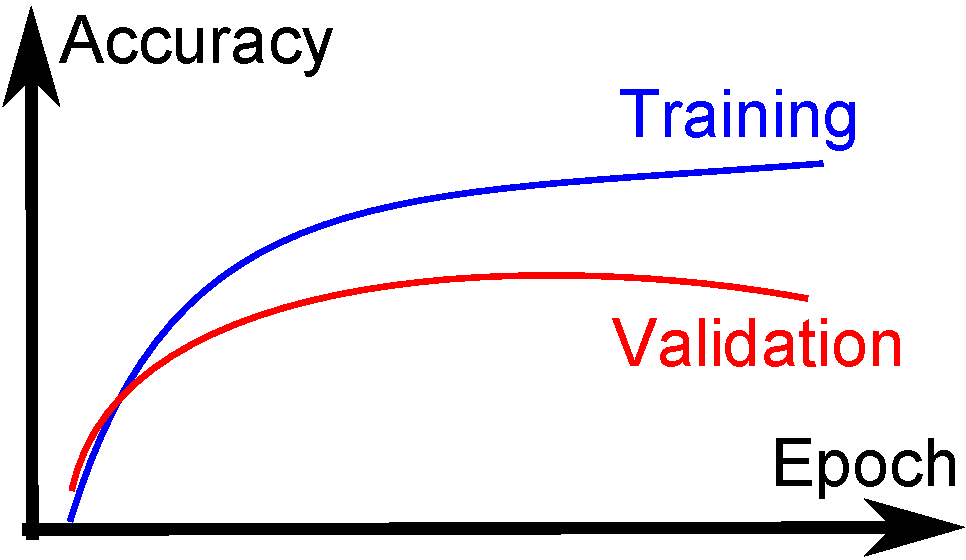
\includegraphics[width=.9\textwidth]{Figures/overfitting.pdf} 
%\end{figure}
%
%\end{column}
%\end{columns}
%
%\end{block}
%
%
%\end{frame}


\begin{frame}
\frametitle{Training and Validation}
\only<2>{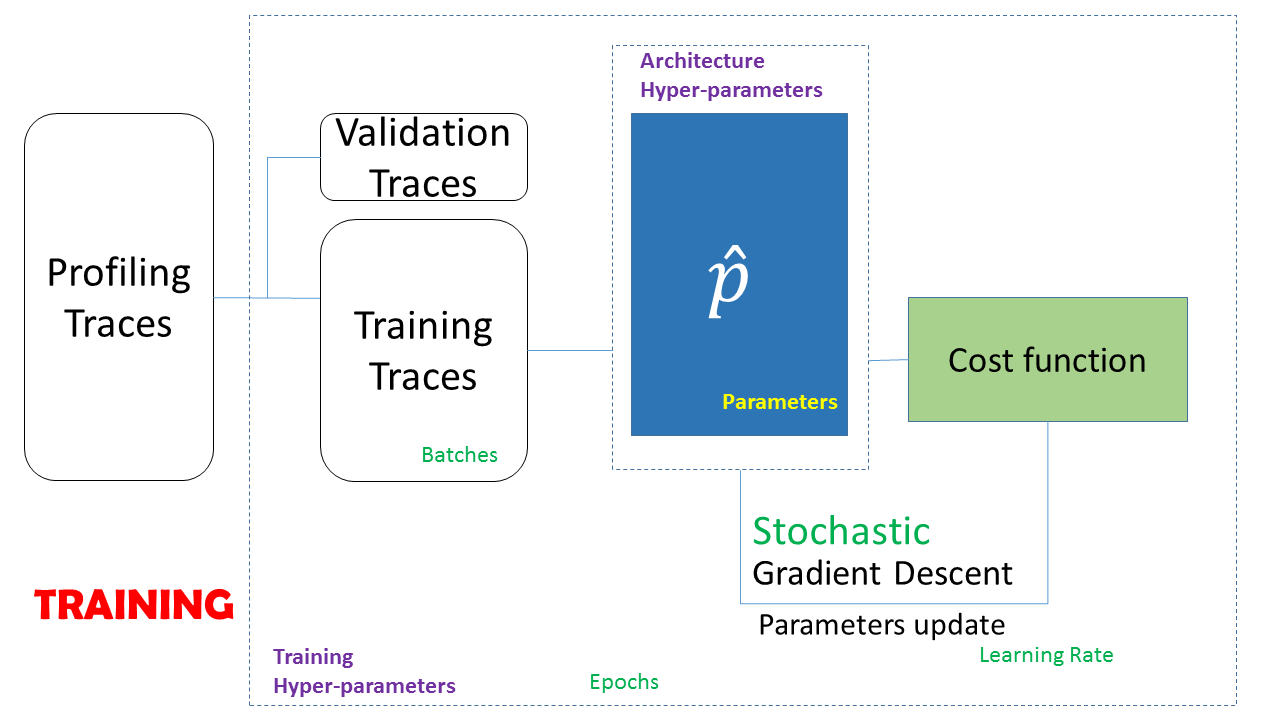
\includegraphics[width=\textwidth]{figures/deep_learning/Diapositive2.PNG}}
\only<3>{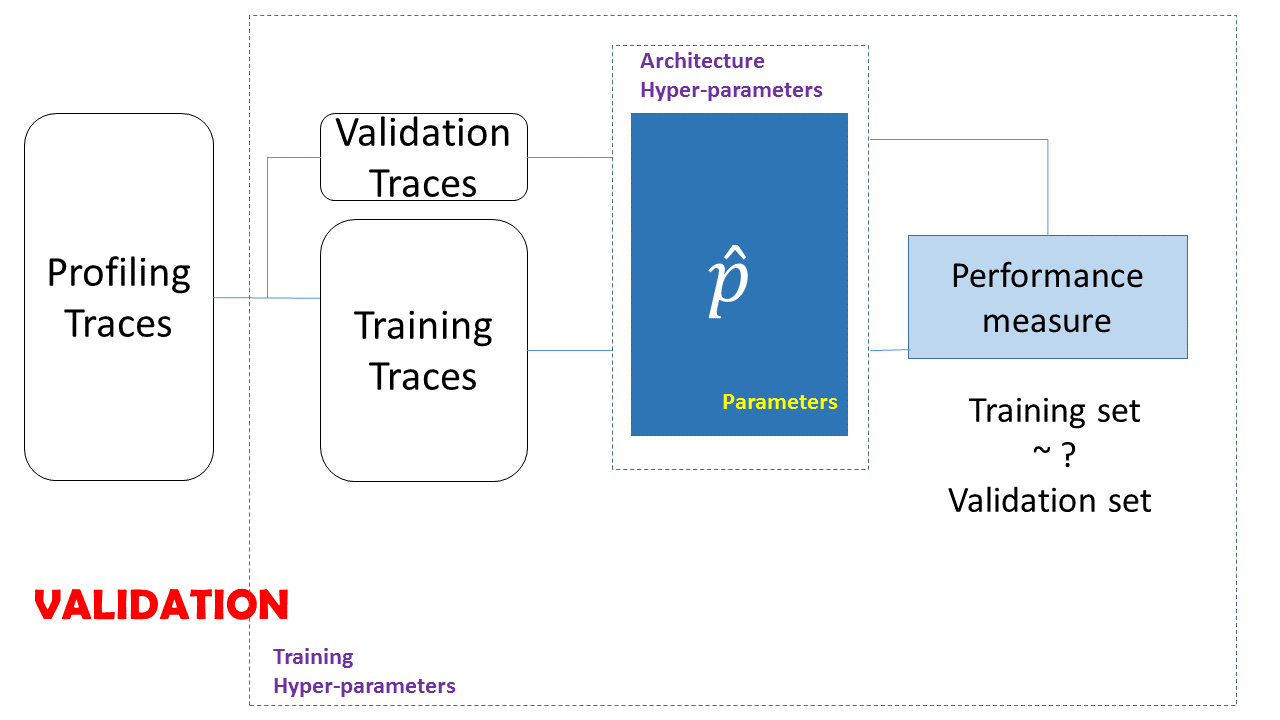
\includegraphics[width=\textwidth]{figures/deep_learning/Diapositive3.PNG}}
\end{frame}


\begin{frame}

\frametitle{Overfitting}

\begin{block}{ Evaluate and compare training and validation accuracy}
\begin{columns}
\begin{column}{.45\textwidth}
\only<2>{Understand significant features
\begin{figure}
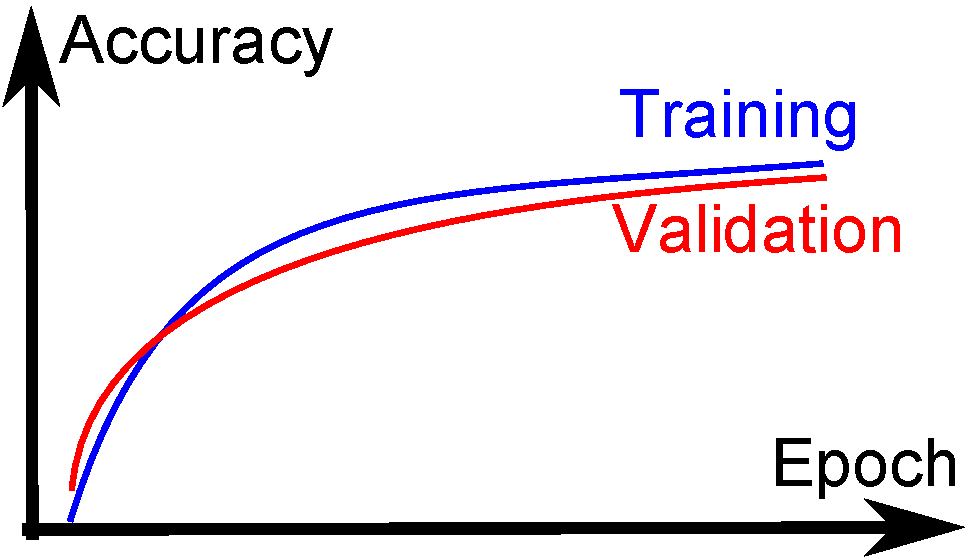
\includegraphics[width=.9\textwidth]{Figures/fitting.pdf} 
\end{figure}
}
\only<3>{
Why?
\begin{itemize}
\item[] Too complex model
\item[] Not enough training data
\end{itemize}
Solution? 
\begin{itemize}
\item[] Data augmentation
\end{itemize}
}
\end{column}
\begin{column}{.45\textwidth}
Learn by heart (\textbf{\textcolor{red}{OVERFITTING}})
\begin{figure}
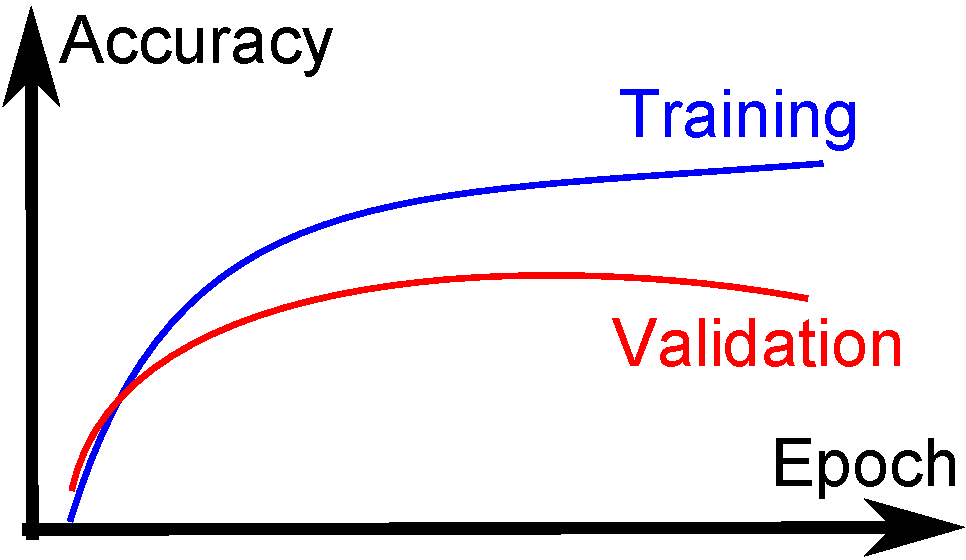
\includegraphics[width=.9\textwidth]{Figures/overfitting.pdf} 
\end{figure}

\end{column}
\end{columns}

\end{block}


\end{frame}

%


\subsection{Data Augmentation}
\begin{frame}
\frametitle{Data Augmentation}
\vspace{-11pt}
\begin{block}{Data Augmentation}
Artificially generate new training data by deforming those previously acquired,
Applying transformations that preserve the label $\sensRandVar$
\end{block}
\vspace{-5pt}
\begin{block}{Countermeasure Emulation Idea}
Emulate the effects of misaligning countermeasures to generate new traces
\begin{columns}
\begin{column}{0.35\textwidth}
\begin{large}
\textbf{\textcolor{green}{SHIFTING}}
\vspace{-8pt}
\end{large}
\end{column}
\begin{column}{0.35\textwidth}
\begin{large}
\textbf{\textcolor{blue}{ADD-REMOVE}}
\vspace{-8pt}
\end{large}
\end{column}
\end{columns}
\begin{figure}
  \begin{minipage}[b]{0.5\linewidth}
    \centering
    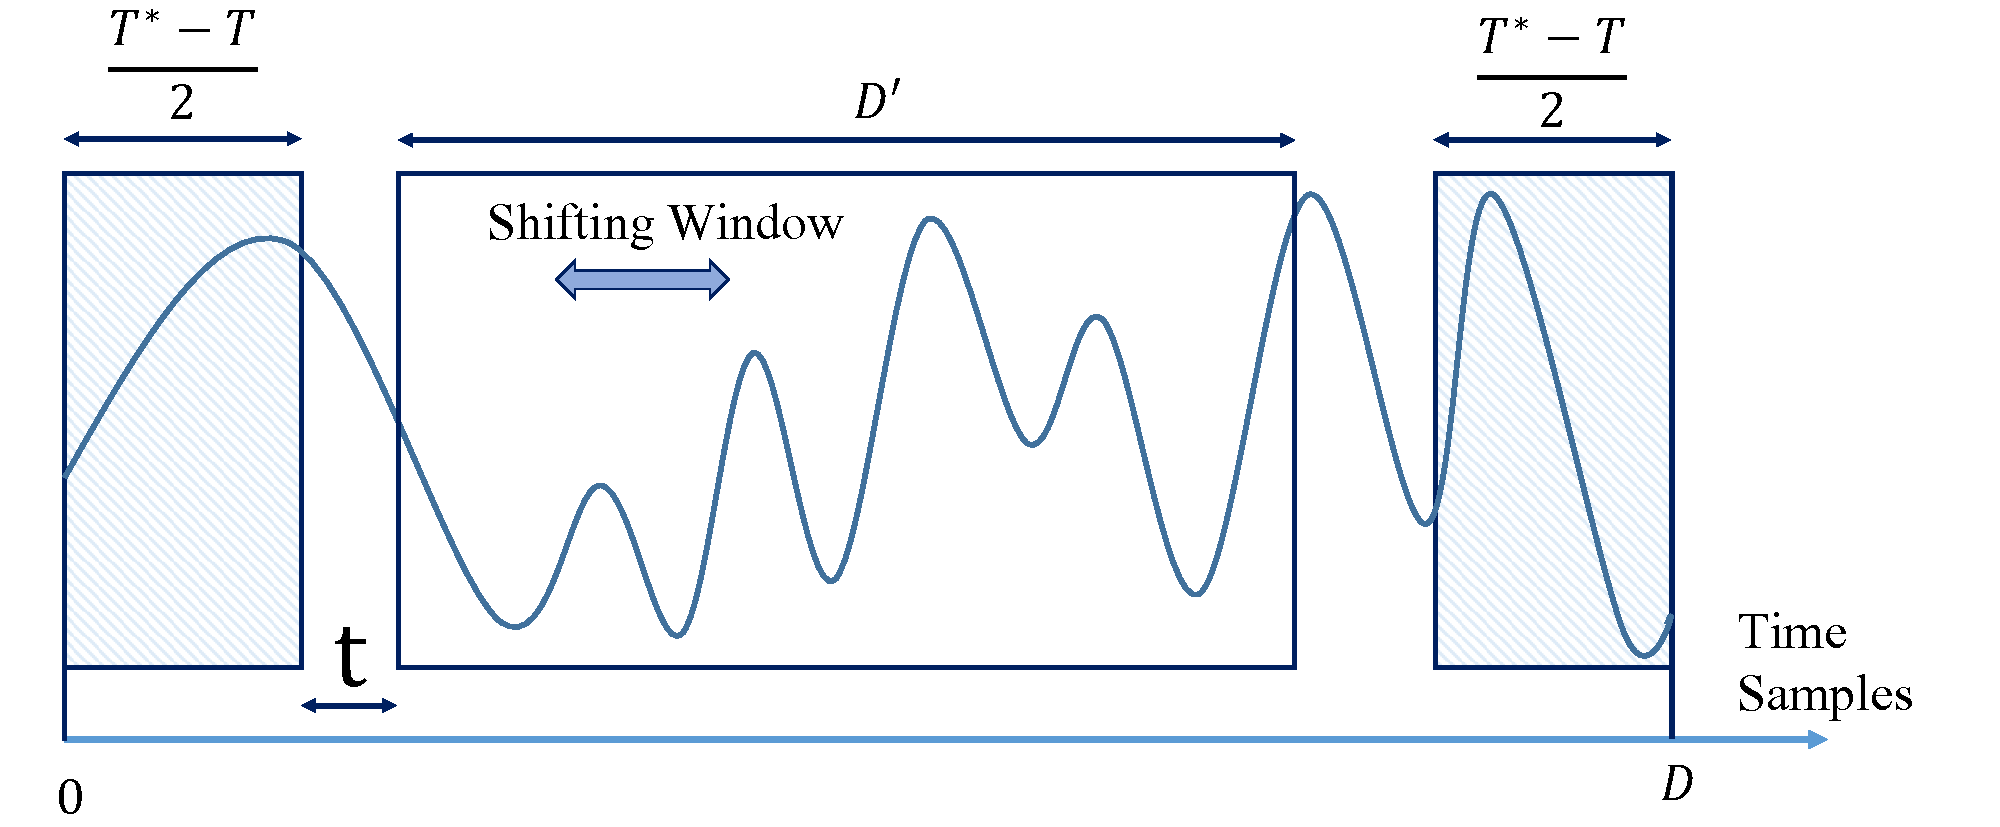
\includegraphics[width=\linewidth]{../Figures/CHES2017/Shifting_window.pdf} 
    \caption{\textcolor{green}{$SH_T$}}
  \end{minipage}%%
  \begin{minipage}[b]{0.5\linewidth}
    \centering
    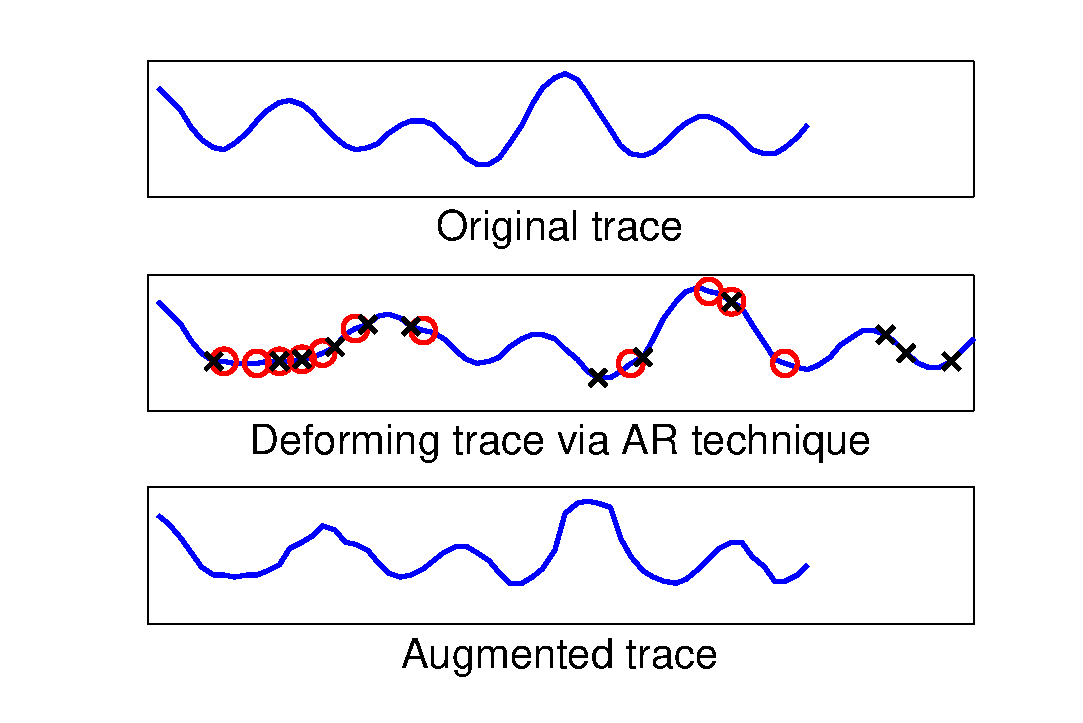
\includegraphics[width=.7\linewidth]{../Figures/CHES2017/AR_example.pdf} 
    \caption{\textcolor{blue}{$AR_R$}}
  \end{minipage} 
\end{figure}
\vspace{-9pt}
Parameter  \textcolor{green}{$T$}: $\sharp$ of possible positions \\
Parameter \textcolor{blue}{$R$}: $\sharp$ of added and removed points \\
Data Augmentation techniques are applied online during training phase.
\end{block}
\end{frame}


\subsection{Experimental Results}
\begin{frame}
\frametitle{Experimental Results}
\begin{itemize}
\item \only<1>{Random delays (software countermeasure)}\only<2>{\textcolor{red}{Random delays (software countermeasure)}}
\item \only<1>{Artificial Jitter (simulated hardware countermeasure)}\only<2>{\textcolor{grey}{Artificial Jitter (simulated hardware countermeasure)}}
\item \only<1>{Real Jitter (hardware countermeasure)}\only<2>{\textcolor{grey}{Real Jitter (hardware countermeasure)}}
\end{itemize}

\vspace*{3pt}
Keras 1.2.1 library with Tensorflow backend \cite{keras} (open source, today 2.2.4)


\end{frame}

\begin{frame}
\vspace*{-5pt}
\frametitle{Random delays}
\vspace{-18pt}
\begin{figure}
\subfloat[One leaking operation]{
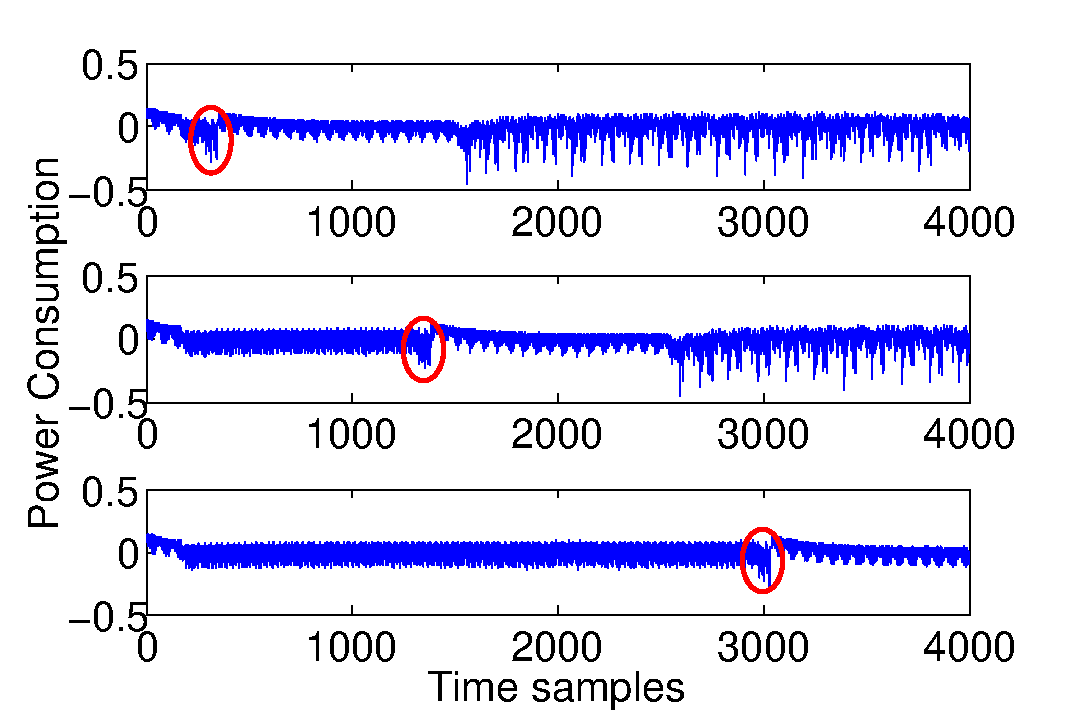
\includegraphics[width=.4\textwidth]{../Figures/CHES2017/CW_shift_traces.pdf} }

\end{figure}
\vspace*{-13pt}
\begin{block}{Setup}

\begin{itemize}
\item Target Chip: Atmega328P 
\item Target Variable: $Z = \mathrm{HW}(\mathrm{Sbox}(P\oplus K))$
\item Acquisition: through \emph{ChipWhisperer}\textregistered\ platform, $\approx 4,000$ time samples
\item Countermeasure: Random Delays - insertion of $r$ \emph{nop} operations, $r \in [0,127]$ uniform random
\item $1,000$ training traces

\end{itemize}
\end{block}


\end{frame}

\begin{frame}
\frametitle{Random delays}
\framesubtitle{Data augmentation vs overfitting}
\vspace{-8pt}
\begin{block}{Metrics}
\begin{itemize}
\item Test accuracy: classification accuracy over the attack traces
\item $N^\star$: minimum number of attack traces to make \emph{guessing entropy} of the right key permanently equal to one ($N^\star$ estimated over 10 independent attacks)
\end{itemize}
\end{block}


\begin{figure}
\captionsetup[subfigure]{labelformat=empty}
\subfloat[\textcolor{green}{$SH_0$}]{
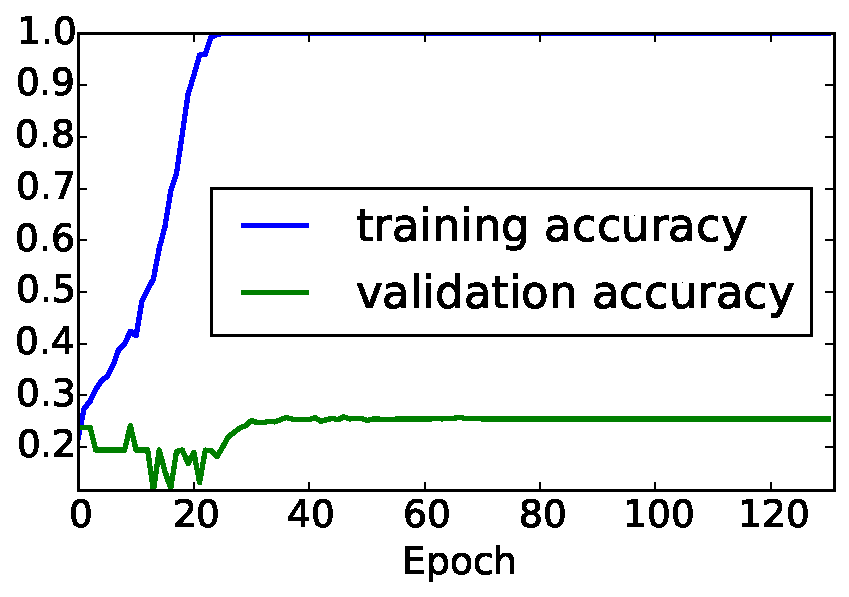
\includegraphics[width=.3\textwidth]{../Figures/CHES2017/DAshift0_2000traces_9classes_sgd/acc_DAshift0_2000traces_9classes_sgd.pdf} 
}
\subfloat[\textcolor{green}{$SH_{100}$}]{
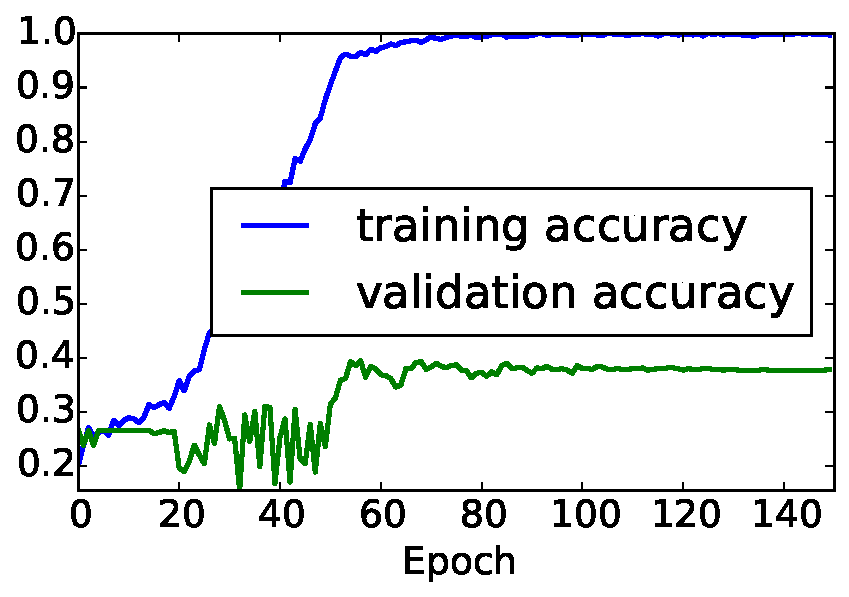
\includegraphics[width=.3\textwidth]{../Figures/CHES2017/DAshift100_2000traces_9classes_sgd/acc_DAshift100_2000traces_9classes_sgd.pdf} 
}
\subfloat[\textcolor{green}{$SH_{500}$}]{
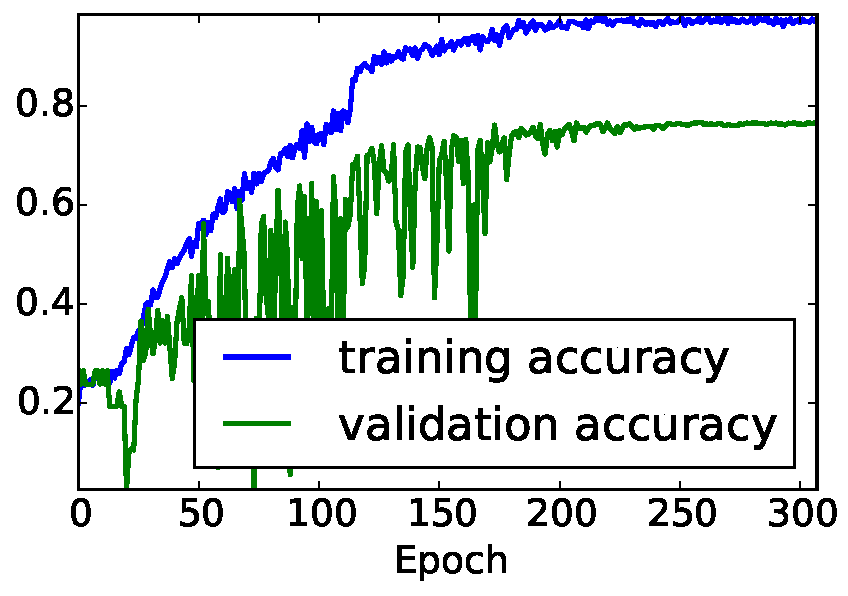
\includegraphics[width=.3\textwidth]{../Figures/CHES2017/DAshift500_2000traces_9classes_sgd/acc_DAshift500_2000traces_9classes_sgd.pdf} 
}
\end{figure}

\pause
\vspace*{-15pt}
\begin{table}
\begin{tabular}{|c|c|c|c|c|c|c|c|}
\multicolumn{8}{c}{}\\
\hline
\multicolumn{2}{|c|}{} & \multicolumn{2}{c|}{\textcolor{green}{$\mathrm{SH}_{0}$}} & \multicolumn{2}{c|}{\textcolor{green}{$\mathrm{SH}_{100}$}} & \multicolumn{2}{c|}{\textcolor{green}{$\mathrm{SH}_{500}$}} \\ \hline
Acc        & $N^\star$       & 27.0\%                      & $>1,000$                      & 31.8\%                       & 101                         & \textbf{78\%}              & \textbf{7}                \\ \hline
\end{tabular}
\end{table}
%
\end{frame}
%



\begin{frame}
\frametitle{Conclusions about CNN}

\begin{block}{}
\begin{itemize}
\item State-of-the-Art Template Attack routine separates resynchronization/dimensionality reduction from characterization \pause
\item CNNs provide an integrated approach to directly construct a discriminative model from rough data \pause
\item CNN models may have high capacity and require plenty of data to be trained \pause 
\item Data Augmentation provides an answer to the lack of data \pause
\item we proposed two Side-Channel-adapted Data Augmentation techniques (inspired by trace misalignment)\pause
\item we verified the effectiveness/efficiency of the CNN+Data Augmentation approach over different sets of misaligned data
\end{itemize}
\end{block}

\end{frame}
